\section{Results}
-- describe pro-time vs pro-route scenarios
-- describe battery capacities
-- describe maximum charge rates
-- describe how route scheduels, delta, and uncontrolled loads come from uta.
-- describe the gaps used in the minimisation algorithms.
\subsection{Comparison with Prior Work}
In this section, we compare the proposed method with a baseline algorithm and a method developed be \textcolor{red}{insert reference to He. et al here}. The baseline method models how bus drivers charge their electric vehicles at the Utah Transit Authority in Salt Lake City, Utah. At UTA, when bus drivers arrive at the station, they refuel their electric buses whenever a charger is available so that the number of charge sessions is maximized. The method from \textcolor{red}{He et al.} works somewhat differently by minimising the cost of energy with respect to the time of use tarrifs $\mu_{e-on}$ and $\mu_{e-off}$.
\par The comparison we observe is given for a 10-bus, 10-charger scenario with a pro-route preference and a single group. Each method was used to compute a charage schedule and the costs from demand, facilities, and energy charges are given in Fig. \ref{fig:results:costComparison}. Note how the baseline algorithm suffers significantly from the demand charges associated with On-Peak Power, and \textcolor{red}{He et al.} incurres additional cost from the facilities charges, indicating that an emphasis on energy charges and habitual charging patterns can be improved.
\par We observe where the differences in cost originate in Fig. \ref{fig:results:totalPower}. Observe how the baseline charge profile achieved the largest 15-minute average power between 19:12 adn 21:36 which is during on-peak hours and consequently yielded the large On-Peak Power charges given in Fig. \ref{fig:results:costComparison}. Additionally, note how the proposed method maintains a relatively flat power profile so that the load is balanced throughout the day which we investigate in Fig. \ref{fig:results:powerPlot}.
\par In Fig. \ref{fig:results:powerPlot}, note how the proposed method produces a bus load that mirrors the uncontrolled load, yielding the flat load profile from Fig. \ref{fig:results:totalPower} which is especially prevalent from 7:12 to 14:24.
\begin{figure}
	\centering
	\makeComparisonBarChartThree{media/11_results/costComparison.csv}{Cost (Dollars)}{Baseline}{He et al.}{Proposed}
	\caption{Cost comparison with prior work}
	\label{fig:results:costComparison}
\end{figure} 

 
\begin{figure*}
	\centering
	\makeComparisonPower{media/11_results/powerPlotfiscal.csv}{media/11_results/powerPlotconsumption.csv}{15-Minute Average Power (kW)}{Proposed}{He et al.}
	\caption{Comparison between uncontrolled and bus loads}
	\label{fig:results:powerPlot}
\end{figure*}


\begin{figure*}
	\centering
	\makeComparisonTotalPower{media/11_results/totalPowerfiscalproTime.csv}{media/11_results/totalPowerconsumptionproTime.csv}{15-Minute Average Power (kW)}{Proposed}{He et al.}
	\caption{15-Minute average power for one day}
	\label{fig:results:totalPower}
\end{figure*}


\subsection{Scalability of an Optimal Solution}
In the previous section, we discussed performance of the proposed method when each program is solved to an optimal solution. In general, the most computationally demanding solution addressed bus-to-charger placement and generally requries a gap of $1\times10^{-5}$ for optimality. This work also seeks to address how to compute a solution in a scalable manner and so this section reviews computational time as the number of buses increases. Fig. \ref{fig:results:scalabilityTimeVsGap} shows how the computational time scales with the gap from the the program which solves the bus-to-charger assignment problem. Note how the computational time significantly increases as the gap decreases, a phenomena which is exacerbated as the bus-to-charger ratio increases. However, note that even the larger gap values are relatively low, usually around 0.6\%, indicating that we may be able to manage the computational time by significantly increasing the threshold for gaps. 
\begin{figure}
	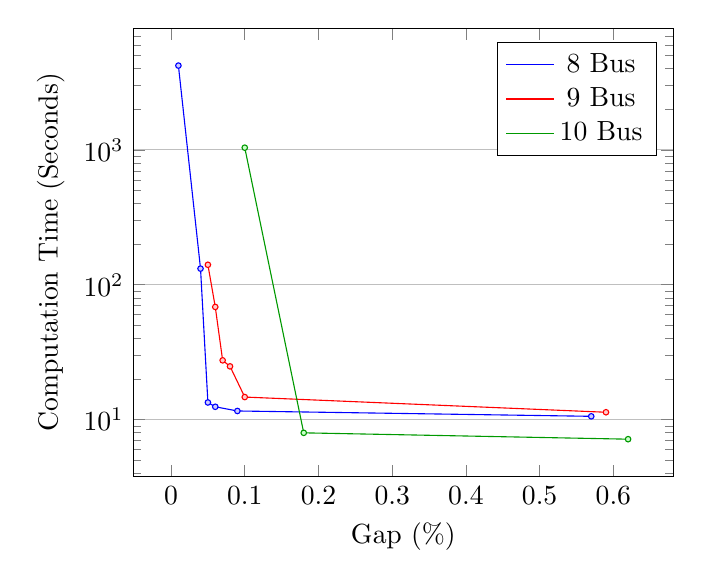
\begin{tikzpicture}
		\begin{axis}[ymajorgrids=true, ylabel={Computation Time (Seconds)}, ymode=log, xlabel={Gap (\%)}, legend pos=north east]%, xtick={0.1, 0.05, 0.01, 0.005, 0.001, 0.0005, 0.0001, 0.00005, 0.00001, 0.000005, 0.000001}, xticklabels={$1\times10^{-1}$, $5\times10^{-2}$, $1\times10^{-2}$, $5\times10^{-3}$, $1\times10^{-3}$, $5\times10^{-4}$, $1\times10^{-4}$, $5\times10^{-5}$, $1\times10^{-5}$, $5\times10^{-6}$, $1\times10^{-6}$}]
			\addplot[blue] coordinates {
				(0.57, 10.58)
				(0.09, 11.59)
				(0.06, 12.45)
				(0.05, 13.40)
				(0.04, 131.78)
				(0.01, 4223.25)
			};
			\addplot[red] coordinates {
				(0.59, 11.34)
				(0.10, 14.70)
				(0.08, 24.83)
				(0.07, 27.51)
				(0.06, 68.49)
				(0.05, 140.70)
			};
			\addplot[green!60!black] coordinates {
				(0.62, 7.16)
				(0.18, 7.98)
				(0.10, 1039.33)
			}; 
			\addplot[fill=blue!20, draw=blue, only marks, mark size=1pt] coordinates {
				(0.57, 10.58)
				(0.09, 11.59)
				(0.06, 12.45)
				(0.05, 13.40)
				(0.04, 131.78)
				(0.01, 4223.25)}; 
			\addplot[fill=red!20, draw=red, only marks, mark size=1pt] coordinates {
				(0.59, 11.34)
				(0.10, 14.70)
				(0.08, 24.83)
				(0.07, 27.51)
				(0.06, 68.49)
				(0.05, 140.70)
			}; 
			\addplot[fill=green!20, draw=green!60!black, only marks, mark size=1pt] coordinates{
				(0.62, 7.16)
				(0.18, 7.98)
				(0.10, 1039.33) 
			};
	\legend{8 Bus, 9 Bus, 10 Bus};
		\end{axis}
	\end{tikzpicture}
	\caption{Comparison of Runtime for a 7-Charger Scenario}
	\label{fig:results:scalabilityTimeVsGap}
\end{figure}



\subsection{Contention: Sub-Optimal Schedules}
In the previous section we observed that a scalable solution the bus charge problem will require that we must either maintain loose gap requirements for the bus-to-charger placement problem, or decrease the computational complexity. In this section, we show that even though a gap may be small for the bus-to-charger problem, the resulting solution may still be undesireable. 
\par Compare the two charge schedules in Fig. \ref{fig:results:disoptimalRoutes} and Fig. \ref{fig:results:optimalRoutes} where Fig. \ref{fig:results:disoptimalRoutes} represents a charge schedule for an arbitrary gap and Fig. \ref{fig:results:optimalRoutes} represents a solution for a gap of $1\times10^{-6}$. In each figure, the color for the i,j location represents the charge rate for bus $i$ at time $j$. Note how the charge sessions in Fig. \ref{fig:results:optimalRoutes} are spread over larger time intervals and contain lower charge rates, which is advantagous because larger time intervals are less challenging from an operational perspective, and the corresponding decrease in immediate power is easier for charging hardware to execute. Therefore, if high performance is necessary, then the effective computational complexity of the bus-to-charger placement problem must be managed.
\input{media/11_results/disoptimalRoutes.tex}
\input{media/11_results/sessionImageStyle}
\begin{figure*}
\begin{tikzpicture}
\begin{axis}[colorbar, ChargeSessionImage, width=0.95\textwidth, height=0.5\textwidth, point meta min=0, point meta max=350, xmin=0.5, xmax=4320.5,xtick={540, 1080, 1620, 2160, 2700, 3240, 3780, 4320}, xticklabels={3:00, 6:00, 9:00, 12:00, 15:00, 18:00, 21:00, 0:00}, ymin=0.5, ymax=18.5]

\addplot [forget plot] graphics [xmin=0.5, xmax=4320.5, ymin=0.5, ymax=18.5] {media/11_results/optimalRoutes-1.png};
\end{axis}

\end{tikzpicture}%
\caption{Routes with a small gap in the route placement problem}
\label{fig:results:optimalRoutes}
\end{figure*}
 

\subsection{The Importance of Groups}
For scenarios where ideal schedules are necessary, we show that the effective computational time can be decreased by separating buses and chargers into groups and solving each sub-problem separately. In this section, we consider a 18 bus, 12 charger scenario with a 0.13\% gap in the bus-to-charger assignment problem where a solution for each scenario is computed after separating the buses and chargers into one and two groups as described in Section \ref{sec:scalability}. Note how the computational time significantly decreases with the addition of a single group, demonstrating how a small number of groups can decrease the runtime for a more optimal solution.
\begin{figure}
\centering
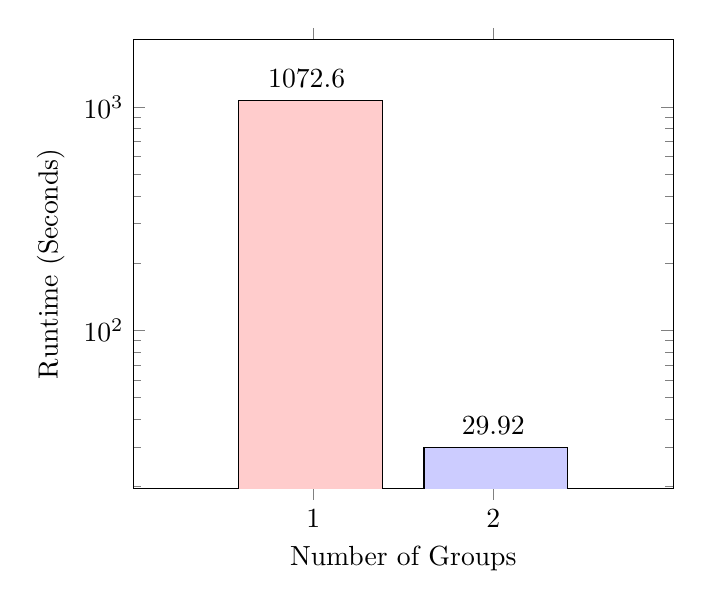
\begin{tikzpicture}
	\begin{axis}[ybar, ymode=log, ymax=2000, xmin=0, xmax=3, xtick={1,2}, xlabel=Number of Groups, ylabel=Runtime (Seconds)]
		\addplot[fill=red!20, bar width=0.8] coordinates {(1.4, 1072.6)};
		\addplot[fill=blue!20, bar width=0.8]  coordinates {(1.6, 29.92)};
	\end{axis}
	\node at (2.2,5.2){1072.6};
	\node at (4.57, 0.79){29.92};
\end{tikzpicture}
\caption{Runtimes for a 18 bus 12 charger scenario at a 0.13\% gap}
\label{fig:results:groupResults}
\end{figure}
 
\subsection{Effects of De-Fragmentation}
This paper also addresses the operational preference of smaller numbers of charge sessions when possible. This section demonstrates the effectiveness the defragmentation method given in Section \ref{sec:defragmentation}, and the overall change in monthly cost. In section \ref{sec:defragmentation}, the threshold for defragmentation is given by the minimum energy allowed per charge session. In this section we consider a scenario with a minimum energy of 0 kWh as shown in Fig. \ref{fig:results:noFragmentationChargeLimit}, and a second at 30 kWh as shown in Fig. \ref{fig:results:defragmentedChargeLimit}. Observe how the many charge sessions are condensed so that each bus must only charge a small number of times. 
\par In Fig. \ref{fig:results:defragmentationCostProTime}, we show the cost remains relatively consistent over a large window of minimum energy thresholds. Computation time also behaves as expected, where larger threshold values result in larger runtimes. However, these runtimes can be managed in the same way as the runtimes for the bus-to-charger placement problem by dividing the buses into groups. Because defragmentation reduces the number of charge sessions, the number of binary variables in the bus-to-charger assignment problem is also reduced so that smaller gaps can be achieved in reduced runtimes.
display heat map of before and after for contested case. 
\begin{figure*}
\centering
\begin{tikzpicture} 
\begin{axis}[colorbar, ChargeSessionImage, width=5.2in, height=2in, point meta min=0, point meta max=350, xmin=0.5, xmax=4320.5, xtick={540, 1080, 1620, 2160, 2700, 3240, 3780, 4320}, xticklabels={3:00, 6:00, 9:00, 12:00, 15:00, 18:00, 21:00, 0:00}, ymin=0.5, ymax=40.5]
\addplot [forget plot] graphics [xmin=0.5, xmax=4320.5, ymin=0.5, ymax=40.5] {\rootdirectorythree/media/11_results/defragmentedChargeLimit-1.png}; 
\end{axis} 
\end{tikzpicture}
\caption{Routes with De-Fragmentation}
\label{fig:results:defragmentedChargeLimit}
\end{figure*}

\begin{figure*}
\centering
\begin{tikzpicture} 
\begin{axis}[colorbar, ChargeSessionImage, width=0.95\textwidth, height=0.5\textwidth, point meta min=0, point meta max=350, xmin=0.5, xmax=4320.5, xtick={540, 1080, 1620, 2160, 2700, 3240, 3780, 4320}, xticklabels={3:00, 6:00, 9:00, 12:00, 15:00, 18:00, 21:00, 0:00}, ymin=0.5, ymax=40.5]
\addplot [forget plot] graphics [xmin=0.5, xmax=4320.5, ymin=0.5, ymax=40.5] {media/11_results/noFragmentationChargeLimit-1.png}; 
\end{axis} 
\end{tikzpicture}
\caption{Routes without De-Fragmentation}
\label{fig:results:noFragmentationChargeLimit}
\end{figure*}
 
\begin{figure}\centering
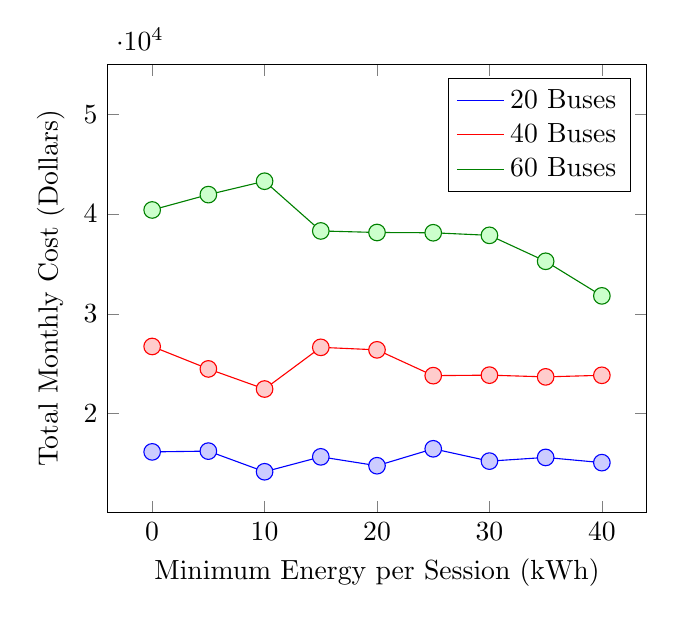
\begin{tikzpicture}
\begin{axis}[xlabel=Minimum Energy per Session (kWh), ylabel=Total Monthly Cost (Dollars), ymax=55000, legend pos=north east]
	\addplot[blue] coordinates {
		(0, 16183.79)   
	  (5, 16260.98)  
		(10,14194.10)  
		(15,15686.16)  
		(20,14798.53)  
		(25,16492.56)  
		(30,15259.19)  
		(35,15628.38)  
		(40,15106.82)};
\addplot[red] coordinates {
		(0, 26738.71)
		(5, 24491.03)
	  (10,22476.88)
		(15,26650.71)
		(20,26400.31)
		(25,23816.91)
		(30,23866.55)
		(35,23693.25)
		(40,23851.78)};
\addplot[green!50!black] coordinates {
		(0, 40405.72)
		(5, 41942.45)
	  (10,43284.09)
		(15,38304.96)
		(20,38150.28)
		(25,38122.51)
		(30,37864.79)
		(35,35268.11)
		(40,31805.12)};

\addplot[blue!20, draw=blue, only marks, mark size=3pt] coordinates {
		(0, 16183.79)  
		(5, 16260.98)  
	  (10,14194.10)  
		(15,15686.16)  
		(20,14798.53)  
		(25,16492.56)  
		(30,15259.19)  
		(35,15628.38)   
		(40,15106.82)};
\addplot[red!20, draw=red, only marks, mark size=3pt] coordinates {
	(0, 26738.71)  	
	(5, 24491.03)  	
	(10,22476.88)   
	(15,26650.71)  	
	(20,26400.31)  	
	(25,23816.91)  	
	(30,23866.55)  	
	(35,23693.25)  	
	(40,23851.78)};	
\addplot[green!20, draw=green!50!black, only marks, mark size=3pt] coordinates {
	(0, 40405.72)  
	(5, 41942.45)  
	(10,43284.09)  
	(15,38304.96)  
	(20,38150.28)  
	(25,38122.51)  
	(30,37864.79)  
	(35,35268.11)  
	(40,31805.12)};

\legend{20 Buses, 40 Buses, 60 Buses} 
\end{axis}
\end{tikzpicture}
\caption{Cost comparison of different degragmentation thresholds in a pro-time optimization scheme.}
\label{fig:results:defragmentationCostProTime}
\end{figure}

\begin{figure}
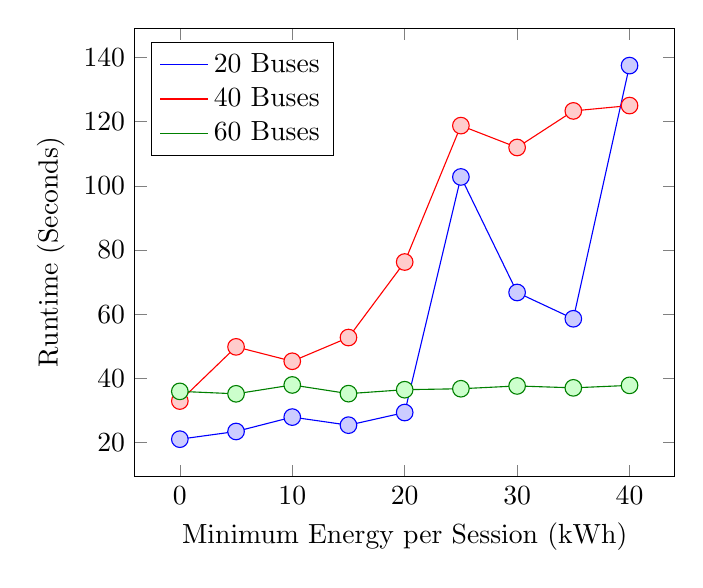
\begin{tikzpicture}
\begin{axis}[xlabel=Minimum Energy per Session (kWh), ylabel=Runtime (Seconds), legend pos=north west]
	\addplot[blue] coordinates {
		(0, 21.00)
		(5, 23.40)
	  (10,27.89)
		(15,25.37)
		(20,29.31)
		(25,102.78)
		(30,66.75)
		(35,58.55)
		(40,137.51)}; 
\addplot[red] coordinates {
		(0, 32.89)
		(5, 49.79)
	  (10,45.30)
		(15,52.70)
		(20,76.25)
		(25,118.79)
		(30,111.97)
		(35,123.37)
		(40,125.04)}; 
\addplot[green!50!black] coordinates {
		(0, 35.91)
		(5, 35.15)
	  (10,37.91)
		(15,35.20)
		(20,36.43)
		(25,36.73)
		(30,37.60)
		(35,37.01)
		(40,37.78)}; 
\addplot[blue!20, draw=blue, only marks, mark size=3pt] coordinates {
		(0, 21.00)
		(5, 23.40)
	  (10,27.89)
		(15,25.37)
		(20,29.31)
		(25,102.78)
		(30,66.75)
		(35,58.55)
		(40,137.51)}; 
\addplot[red!20, draw=red, only marks, mark size=3pt] coordinates {
		(0, 32.89)
		(5, 49.79)
	  (10,45.30)
		(15,52.70)
		(20,76.25)
		(25,118.79)
		(30,111.97)
		(35,123.37)
		(40,125.04)}; 
\addplot[green!20, draw=green!50!black, only marks, mark size=3pt] coordinates {
		(0, 35.91)
		(5, 35.15)
	  (10,37.91)
		(15,35.20)
		(20,36.43)
		(25,36.73)
		(30,37.60)
		(35,37.01)
		(40,37.78)}; 
\legend{20 Buses, 40 Buses, 60 Buses}		
\end{axis}
\end{tikzpicture}
\caption{Comparison of runtime for the uncontested and contested scenarios over different de-fragmentation criteria}
\label{fig:results:runtimeDefragmentation}
\end{figure}

\subsection{Scalability}
In this section, we consolidate what we have learned in the previous sections to demonstrate how the proposed framework can be used to compute a scalable and cost effective solution for large numbers of buses. This section focuses on a scenario with a minimum energy per session of 20 kWh, an arbitrary gap for the bus-to-charger assignment solution, and a single group.
\par The results given in Fig. \ref{fig:results:scalabilityRuntimes} show a a runtime that generally increases by one second per bus.  One would expect the runtime to increase at least on the order of $O(n^2)$ for a globally optimal solution because of the coupling between bus variables. The fact that the proposed method appears linear on the given range indicates a scalable solution. 
\par Generally, one would also expect such savings to come with significant increases to the monthly cost. The results in Fig. \ref{fig:results:scalabilityCosts} however demonstrate how the proposed solution yields a quasi-linear increase of \$404.10 dollars per bus per month. 
\begin{figure}
\centering
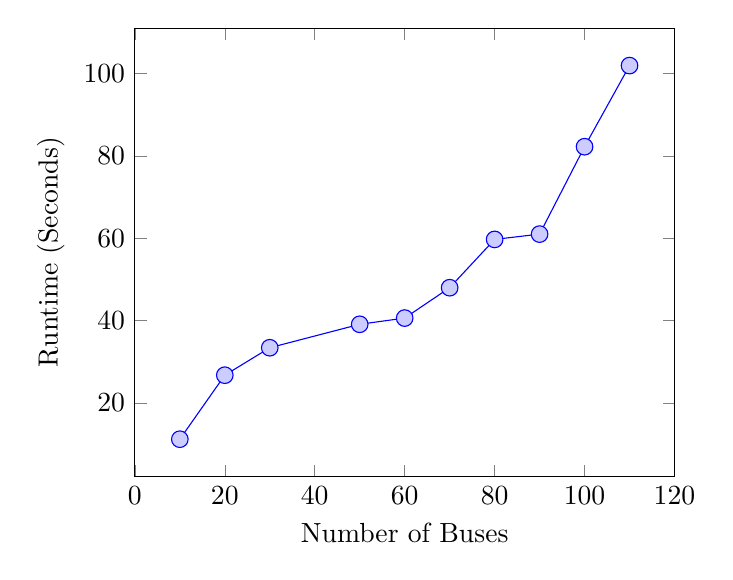
\begin{tikzpicture}
\begin{axis}[xlabel=Number of Buses, ylabel=Runtime (Seconds), legend pos=north west]
	\addplot[blue] coordinates {
		(10, 11.18)   
	  (20, 26.74)  
		(30, 33.41)  
		(50, 39.11)  
		(60, 40.62)  
		(70, 48.00)  
		(80, 59.74)  
		(90, 61.03)
		(100, 82.27)
		(110, 101.99)}; 
\addplot[blue!20, draw=blue, only marks, mark size=3pt] coordinates {
		(10, 11.18)   
	  (20, 26.74)  
		(30, 33.41)  
		(50, 39.11)  
		(60, 40.62)  
		(70, 48.00)  
		(80, 59.74)  
		(90, 61.03)
		(100, 82.27)
		(110, 101.99)};
\end{axis}
\end{tikzpicture}
\caption{Runtime comparison for different numbers of buses}
\label{fig:results:scalabilityRuntimes}
\end{figure}

\begin{figure}
\centering
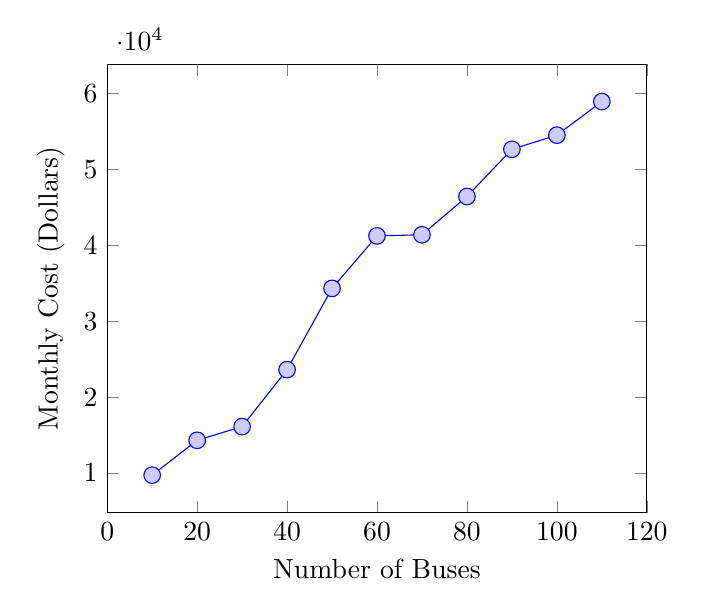
\begin{tikzpicture}
\begin{axis}[xlabel=Number of Buses, ylabel=Monthly Cost (Dollars), legend pos=north west]
	\addplot[blue] coordinates {
		(10, 9724.43)   
	  (20, 14312.58)  
		(30, 16113.51)  
		(40, 23617.81)
		(50, 34317.80)  
		(60, 41226.07)  
		(70, 41374.21) 
		(80, 46412.54)  
		(90, 52628.26)
		(100, 54490.15) 
		(110, 58912.91)}; 
\addplot[blue!20, draw=blue, only marks, mark size=3pt] coordinates {
		(10, 9724.43)   
	  (20, 14312.58)  
		(30, 16113.51)  
		(40, 23617.81)
		(50, 34317.80)  
		(60, 41226.07)  
		(70, 41374.21)  
		(80, 46412.54)  
		(90, 52628.26)
		(100, 54490.15) 
		(110, 58912.91)}; 
\end{axis}
\end{tikzpicture}
\caption{Cost comparison for different numbers of buses}
\label{fig:results:scalabilityCosts}
\end{figure}

	
	
